\documentclass[dvipdfmx]{standalone}
\usepackage{tikz}
\usetikzlibrary{positioning}

\begin{document}
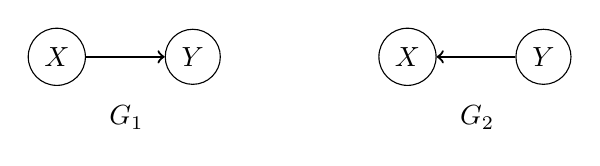
\begin{tikzpicture}[
  nodestyle/.style={
        draw,
        circle
  }
]

    \coordinate (G) at (0cm, 0cm);

    \node[nodestyle] (X_1) {$X$};
    \node[nodestyle, right=1cm of X_1] (Y_1) {$Y$}
    node[below left = 0.5cm and 0.5cm of Y_1.center]{$G_1$};

    \node[nodestyle, right=2cm of Y_1] (X_2) {$X$};
    \node[nodestyle, right=1cm of X_2] (Y_2) {$Y$}
    node[below left = 0.5cm and 0.5cm of Y_2.center]{$G_2$};

    \draw[thick, ->] (X_1) -- (Y_1);
    \draw[thick, ->] (Y_2) -- (X_2);
\end{tikzpicture}
\end{document}
